% !TEX root = ../Thesis.tex

%front matter =============================================================
%\pagestyle{plain}
\frontmatter
%titlepage ---------------------------------------------------------------------
\hypersetup{pageanchor=false}
\begin{titlepage}

\begin{center}

\begin{figure}[!ht]

\includegraphics[height=12mm]{ethlogo}
\hfill
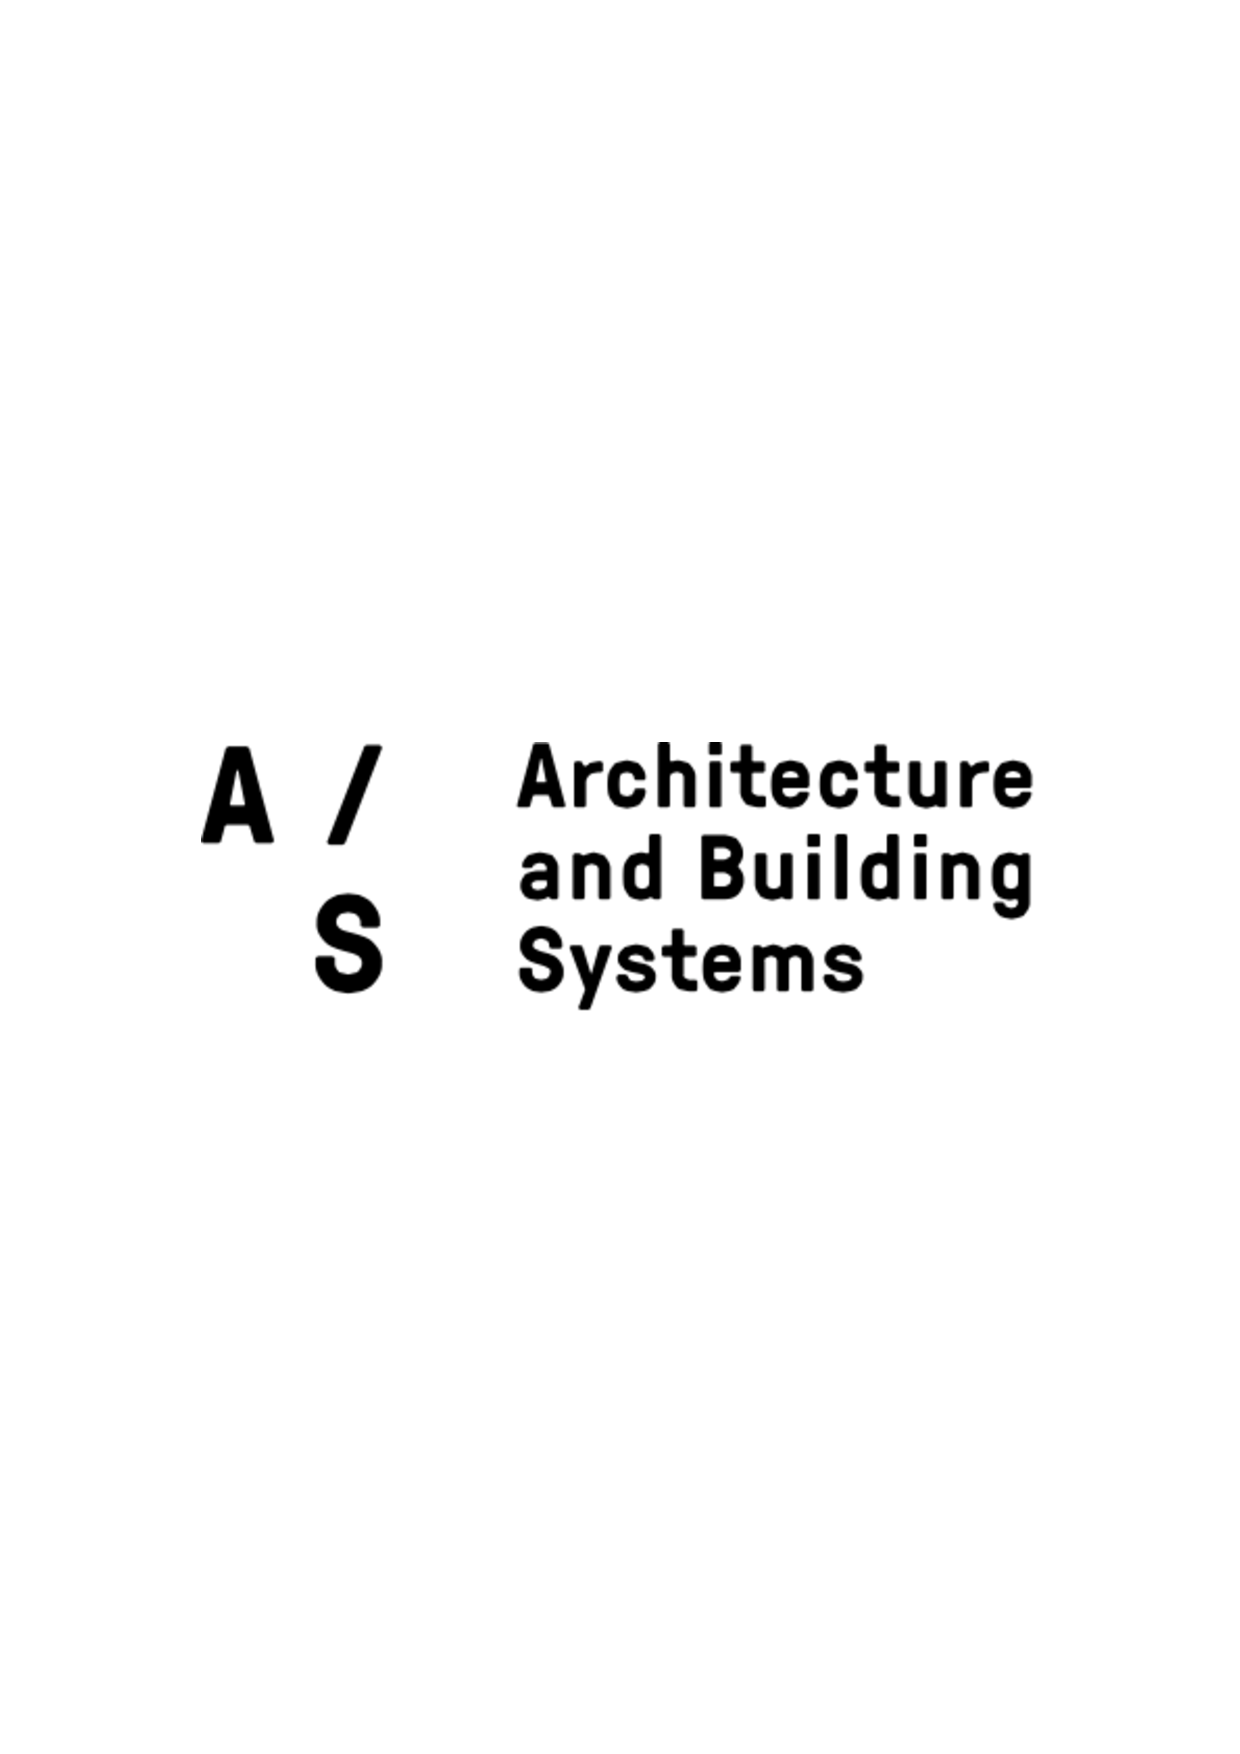
\includegraphics[height=12mm]{ASlogo}
\end{figure}

\vspace{30mm} 

Justin Zarb \\

\vspace{10mm} 
\begin{doublespace}
\textbf{\LARGE Design of a simplified Resistor-Capacitor Model} \\
\end{doublespace}

\vspace{10mm} 

Semester Project \\ 


\vfill

ITA -- Architecture and Building Systems\\ 
Swiss Federal Institute of Technology (ETH) Zurich \\

\vspace{5mm}

\textbf{Examiner:}\\ 
Prof. Dr. Arno Schl\"uter\\

\vspace{5mm} 

\textbf{Supervisors:} \\
Prageeth Jayathissa

\vspace{5mm} Zurich, \today

\end{center}
\end{titlepage}
\hypersetup{pageanchor=true}

%Abstract ---------------------------------------------------------------------

\chapter*{Abstract}
%Write this section last





\clearpage

%Acknowledgements ---------------------------------------------------------------------
\chapter*{Acknowledgements}

I would like to thank PJ for being a really cool guy





\clearpage

\tableofcontents

\newpage

\chapter*{List of Acronyms}
\addcontentsline{toc}{section}{List of Acronyms}
\begin{table}[h]
\begin{tabular}{ll}
AP  & Acidification Potential\\
ASF & Adaptive Solar Facade\\

\end{tabular}\hfill\
\end{table}
\newpage

\listoffigures
\addcontentsline{toc}{section}{List of Figures}
\newpage

\listoftables
\addcontentsline{toc}{section}{List of Tables}

\mainmatter 
